\subsection{MM algorithm}

The \definition{Matrix Multiply (MM) algorithm} consists of three steps:
\begin{enumerate}
    \item \textbf{Compute the two matrices} $A_{i,l}$ and $B_{l,j}$, so use the concurrent read.
    \item Make the \textbf{sum}.
    \item \textbf{Store} the result using exclusive write.
\end{enumerate}
\begin{lstlisting}[mathescape=true, caption={Matrix Multiply (MM)}]
BEGIN
    $T_{i,j,l}$ = $A_{i,l} B_{l,j}$
    FOR = H = 1 : K
        IF $l \le n \div 2^{h}$ THEN
            $T_{i,j,l}$ = $T_{i,j,2l-1}$ + $T_{i,j,2l}$
    IF $l = 1$ THEN
        $C_{i,j}$ = $T_{i,j,1}$
END
\end{lstlisting}
\begin{flushleft}
    \textcolor{Green3}{\faIcon{tachometer-alt} \textbf{Performance of MM}}
\end{flushleft}
\begin{itemize}
    \item $T_{1} = n^{3}$
    \item $T_{p = n^{3}} = \log n$
    \item $\mathrm{SU} = \dfrac{n^{3}}{\log n}$
    \item $\text{Cost} = n^{3} \log n$
    \item $E_{p} = \dfrac{T_{1}}{pT_{p}} = \dfrac{1}{\log n}$
\end{itemize}
\begin{figure}[!htp]
    \centering
    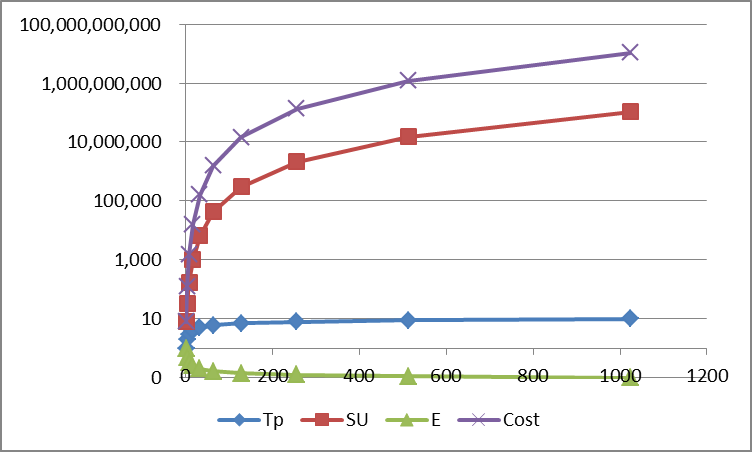
\includegraphics[width=.6\textwidth]{img/mm-1.png}
\end{figure}